\documentclass[letter,10pt]{article}
\usepackage[utf8]{inputenc}
\usepackage[spanish, activeacute]{babel}
\usepackage{geometry}
\geometry{verbose,tmargin=0cm,bmargin=2cm,lmargin=2cm,rmargin=2cm,headheight=0cm,headsep=1cm,footskip=1cm}
\usepackage{graphicx}


%%%%%%%%%%%%%%%%%%%%%%%%%%%%%% Textclass specific LaTeX commands.
\newcommand{\lyxaddress}[1]{
\par {\raggedright #1
\vspace{1.4em}
\noindent\par}
}

%%%%%%%%%%%%%%%%%%%%%%%%%%%%%% User specified LaTeX commands.
\date{}

\begin{document}

\title{Problema C - Cortando Pizza}


\includegraphics[scale=0.6]{logo} \hspace*{9.00cm}

\includegraphics[scale=0.5]{dsc} 
\bigskip
\begin{center}
	\Large Problema C - Cortando Pizza
\end{center}

\begin{flushright}
Límite de tiempo: 3 segundos
\par\end{flushright}
\bigskip

\section*{Problema}

Ricardo dice ser muy inteligente y que su inteligencia y perspicacia le ayudarán en todo. Él dice que si su inteligencia le permite hacer una actividad realizando un esfuerzo físico menor ¿Por qué debe de cansarse más de la cuenta?. También él dice que si usa su cerebro para realizar un menor esfuerzo no es por holgazanería sino una muestra elegante de su superioridad intelectual. 

En alguna ocasión Ricardo se preguntó cómo cortar una pizza en siete rebanadas y repartirlas entre sus amigos, para ello el tamaño de las rebanadas puede no ser el mismo. Pensó un poco y llegó a la conclusión de que podía obtener las siete rebanadas realizando sólo tres cortes -de orilla a orilla- a la pizza, con un cortador de pizza. Aquí mostramos la forma en que Ricardo cortó aquella pizza: 

\begin{figure}[h!]
	\centering
	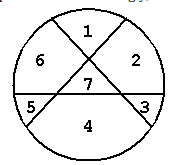
\includegraphics[width=0.20\textwidth]{pizza}
  	\caption{7 rebanadas}
\end{figure}

Uno de sus amigos, quien nunca creyó en la inteligencia de Ricardo, pensó ``Si Ricardo puede hacerlo, ¿Por qué no podría hacerlo mi computadora?''. Así que este amigo intento hacer algo similar (pero no exactamente igual a él porque Ricardo lo criticaría por haberle robado la idea) con ayuda de su computadora. Él escribió un programa que dado el número de cortes en la pizza dice el número máximo de rebanadas que se pueden obtener con exactamente ese número de cortes.

Tu trabajo aquí es escribir un programa similar. Es seguro que el amigo de Ricardo no te criticará por hacer el mismo trabajo que él.

\subsection*{Entrada}

El archivo de entrada contiene un entero por linea $n$ ($0 \leq n \leq 4,295,113,503$) que representa el número de cortes que se deben hacer de lado a lado de la pizza. Un número negativo termina con la entrada.

\subsection*{Salida}

La salida debe ser un entero, el número máximo de rebanadas que se pueden producir.

$$$$
$$$$
$$$$
$$$$
$$$$

\subsection*{Entrada ejemplo}
\noindent \texttt{5}~\\
\texttt{10}~\\
\texttt{-100}~\\
\noindent 

\subsection*{Salida Ejemplo}

\noindent \texttt{16}~\\
\texttt{56}~\\

\noindent \rule[0.5ex]{1\columnwidth}{1pt}


\lyxaddress{UVA Online Judge}
\end{document}
